\documentclass[conference]{IEEEtran}
\IEEEoverridecommandlockouts

\usepackage{cite}
\usepackage{amsmath,amssymb,amsfonts}
\usepackage{algorithmic}
\usepackage{algorithm}
\usepackage{graphicx}
\usepackage{textcomp}
\usepackage{xcolor}
\usepackage{booktabs}
\usepackage{hyperref}
\usepackage{array}

% Path to extracted images folder
\graphicspath{{images/}}

\def\BibTeX{{\rm B\kern-.05em{\sc i\kern-.025em b}\kern-.08em
    T\kern-.1667em\lower.7ex\hbox{E}\kern-.125emX}}

\begin{document}

\title{Resilient Routing in Wireless Mesh Networks using Digital Twin and GNN-Based Reinforcement Learning}

\author{
  \IEEEauthorblockN{Anandakrishnan K V}
  \IEEEauthorblockA{
    \textit{Department of}\\
    \textit{Computer Science and IT,}\\
    \textit{School of Computing,}\\
    \textit{Amrita Vishwa Vidyapeetham, Kochi}\\
    anandakrishnankv23@gmail.com
  }
  \and
  \IEEEauthorblockN{Sreelekshmi S}
  \IEEEauthorblockA{
    \textit{Department of}\\
    \textit{Computer Science and IT,}\\
    \textit{School of Computing,}\\
    \textit{Amrita Vishwa Vidyapeetham, Kochi}\\
    sreelekshmis@kh.amrita.edu
  }
  \and
  \IEEEauthorblockN{Drupad M D}
  \IEEEauthorblockA{
    \textit{Department of}\\
    \textit{Computer Science and IT,}\\
    \textit{School of Computing,}\\
    \textit{Amrita Vishwa Vidyapeetham, Kochi}\\
    drupadmdas@gmail.com
  }
}
\maketitle

%------------------------------------------------------------------
\begin{abstract}
A Wireless Mesh Network (WMN) is a communications network made up of multiple radio nodes organized in a mesh topology used for connecting dynamically with each other. Their flexibility in dynamic connectivity and multi-hop capabilities can attract major threats. Particularly, jamming attacks can severely degrade network performance by disrupting routing and data transmission. Traditional routing protocols lack the adaptability to operate effectively in such dynamic and hostile environments. This article proposes an integrated resilience framework for WMNs that combines digital twin modelling, graph neural networks, and reinforcement learning. A digital twin simulates realistic network behaviour and jamming scenarios, while a GAT model captures the topological and traffic features. A multi-agent deep Q-network utilizes these embeddings to learn adaptive routing strategies under varying jamming conditions.
\end{abstract}

\begin{IEEEkeywords}
Digital twin, routing, jamming detection, DQN, GNN.
\end{IEEEkeywords}

%------------------------------------------------------------------
\section{Introduction}

Wireless communication networks have greatly influenced the advancement of interconnectivity of the technology without a physical medium. Main problem is that the reach of a single wireless device is far less to be suitable for a proper networking. This is where Wireless Mesh Networks (WMNs) fill the gap. WMNs use multi-hop routing. This extends the coverage of data transmission. Multiple nodes are interconnected and take part in a single information transfer. Having a decentralized architecture makes them handy in real-world applications like disaster response, industrial automation, and Internet-of-Things (IoTs). Due to this flexibility, WMNs are also prone to different kind of attacks. These attacks damage the interconnectivity of the nodes, affect network reliability, delays sensitive communication and affect overall Quality-of-Service.

Conventional methods for network resilience include heuristic-based topology control and rule-based routing. These fall short in dynamic environments. Whereas, the mathematical optimization approaches face scalability limitations. Reinforcement Learning (RL) techniques have shown promise in adaptive, real-time decision-making in dynamic environments. However, many such methods still rely on centralized architectures degrades the decentralized nature of WMNs.

To mitigate these problems, this paper proposed a novel approach that integrates three technologies including Digital Twin (DT), Multi-Agent Deep Q-Networks (DQN) and GAT. These three together forms the basis for jamming detection and fault tolerance in resilient WMNs.

Let us now look into these technologies briefly.

\textbf{Digital Twin (DT)} is like a real-time virtual mirror of the real network which helps in the detection of anomalies and analysis of predictive failures. Comparison between the actual and expected radio signals, they are able to detect jamming attacks and analyse their impacts.

\textbf{Multi-Agent DQN} helps to extend traditional reinforcement learning by enabling the nodes to collaboratively adapt their routing and transmission policies. Each node has an agent embedded with it. Each node has an embedded agent that learns to optimize routing performance using its own policy network over a global graph embedding, while sharing experiences across agents through a common replay pool.

\textbf{Graph Attention Network (GAT)} is an attention-based Graph Neural Network (GNN) framework. They are used to extract structural features from the network graph. By aggregating information from neighbouring nodes through learned attention weights, GATs can generate node embeddings which helps in guiding routing decisions. This can also facilitate the detection of anomalies by understanding the global topology.

In short, these components can detect and mitigate threats, and also adapt to the changing network conditions. This will form the basis for a scalable and dynamic routing solution for WMNs.

Recent research in Wireless Mesh Networks (WMNs) have shifted the focus from heuristic protocols to machine learning-oriented approaches. This is mostly driven by the need to handle increasingly complex network dynamics such as mobility of nodes, spectral interference, and dynamic traffic loads. In short, make the whole system dynamic.

\subsection{Routing using Reinforcement Learning and Graph Neural Networks (GNNs)}

Routing in Wireless Mesh Networks (WMNs) is typically modeled as a Markov Decision Process (MDP). This framework allows autonomous agents to develop optimal routing policies by exploring and interacting with their environment.

\textbf{Deep Reinforcement Learning (DRL) and GNNs:} Pappone et al. (2023) introduced a framework that integrates GNNs with Multi-Agent-DRL to overcome a core weakness in traditional Reinforcement Learning: the inability to generalize to unfamiliar network topologies without significant retraining. By leveraging GNNs to encode the network state, their model captures the graph's permutation-invariant structure, enabling agents to minimize flow collisions and adapt to real-time changes.

\textbf{Resilient Emergency Routing:} Jin et al. (2025) proposed Deep Reinforcement Learning-based Resilient Routing (DRLRR) specifically for urban emergency communication networks. Their approach utilizes Double Deep Q-Networks (DDQN) to overcome this bias that is created due to overestimation, which is common in standard Q-learning. This technique precisely detects dynamic topology changes by optimizing message formats and integrating node and link state information into a specialized reward function, ensuring stable data transmission during disasters.
%------------------------------------------------------------------
\section{Related Works}

Recent developments in wireless mesh networks show a clear shift from fixed rule-based protocols to dynamic machine learning-driven techniques. This evolution is driven by the increasing complexity of network dynamics, including challenges such as node mobility, spectral interference, and fluctuating traffic loads.

\subsection{ GNNs and Reinforcement Learning in Routing}

\textbf{Deep Reinforcement Learning (DRLR) and GNNs:} In 2023 Pappone et al. proposed a deep reinforcement learning and GNN model that integrates GNNs multi agent Deep Reinforcement Learning (RL). Their work contributed to one of the core drawback of RL such as generalization to new topologies was limited without retraining over numerous iterations. By encoding the network state using GNN, their model reflects the permutation-invariant structure of the graph, thus enables the agents to minimize flow collisions while adapting to topology changes dynamically.

Similarly in 2025 Jin et al. researched Deep Reinforcement Learning Based Resilient Routing (DRLRR) for urban emergency networks. To counter the overestimation bias of conventional Q-learning, they used Double Deep Q-Networks, enabling them to provide reliable route optimization despite excessive node degradation scenarios.

\textbf{Graph Convolutional Networks (GCN):} gained popularity in 2017 thanks to Kipf and Welling. The objective was for the model to learn on graphs using an efficient spectral approximation of convolution. In this approach, each node's representation is iteratively refined by aggregating the features of its local neighbors, which are then normalized by the degrees of the related nodes. During convolution, the convolutional GCN assumes a constant graph structure and uses only the adjacency of the graph (i.e., structural connectivity) to determine aggregation of weights instead of learnt pairwise significance scores. With this architecture, information on graphs can be encoded in a computationally efficient manner. Formally, a GCN's layer-wise propagation rule is as follows:

\begin{equation}
H^{(l+1)} = \sigma\left(\tilde{D}^{-\frac{1}{2}}\tilde{A}\tilde{D}^{-\frac{1}{2}}H^{(l)}W^{(l)}\right)
\end{equation}

\noindent Where:
\begin{itemize}
    \item $\tilde{A} = A + I_N$ is the adjacency matrix with added self-connections.
    \item $\tilde{D}$ is the degree matrix of $\tilde{A}$.
    \item $W^{(l)}$ is the layer-specific trainable weight matrix.
    \item $\sigma$ is a non-linear activation function (e.g., SELU).
\end{itemize}

\textbf{Graph Attention Network (GAT):} In 2018 Veli\v{c}kovi\'{c} et al. developed GAT which introduces a more detailed architecture that is essential for robust routing. In contrast to GraphSAGE, which gives all neighbours simple equal or fixed weights, GATs obtain attention coefficients $\alpha_{ij}$ by using a self-attention mechanism. $\alpha_{ij}$ shows how important neighbor $j$ is to node $i$.

\begin{equation}
\alpha_{ij} = \frac{\exp\left(\text{LeakyReLU}\left(\vec{a}^T\left[W\vec{h_i} \| W\vec{h_j}\right]\right)\right)}{\sum_{k \in \mathcal{N}_i} \exp\left(\text{LeakyReLU}\left(\vec{a}^T\left[W\vec{h_i} \| W\vec{h_k}\right]\right)\right)}
\label{eq:gat}
\end{equation}

In theory and practice, the GAT architecture handles many of the dynamic features of WMNs more effectively than GCN. Unlike GCN, which assigns uniform weights during aggregation, GAT selectively weights each neighbour's contribution through a learnable attention mechanism, making it particularly suited for environments where link reliability varies due to jamming or interference. This selective aggregation allows GAT to better capture the importance of high-quality, non-jammed links during routing, which is the core motivation for its adoption in this framework.

\subsection{Fault and Anomaly Detection}

Understanding the present condition of the network has a direct impact on routing performance. It is important to determine whether a disruption is the consequence of a routine malfunction or something more intentional before making any routing decisions.

\textbf{Digital Twin for Radio Environments:} What Krause et al. (2023) brought to the table was a rethinking of how anomaly detection works in radio environments. Rather than anchoring detection to patterns mined from past data, their system keeps a physics-based virtual replica of the network running alongside it in real time. A ray-tracing engine inside that replica works out what RSSI readings across each link ought to look like under normal conditions. Those calculated values become references. Any meaningful gap between predicted and measured signals gets flagged — no attack examples needed for training. Crucially, the framework can tell jamming apart from ordinary fading, which is exactly where conventional statistical detection tends to fall apart.

\subsection{Gap Analysis}

Pappone et al. (2023) built a solid routing foundation, yet the work overlooks the subtleties of physical layer threats by anchoring itself to standard network metrics. Krause et al. (2023) take a different angle leveraging digital twins for detection but deliberately stop at observation, leaving the door closed on any form of active network intervention.

Existing work has yet to meaningfully explore the tight integration of these two systems — particularly the idea of feeding high-fidelity anomaly scores from a Digital Twin directly into a Graph Attention Network (GAT) as live, dynamic features. This paper takes a step into that gap. The core proposition is that routing the Digital Twin's ground-truth awareness through the attention mechanism of a GAT-based reinforcement learning agent enables the network to build genuine resilience — one where interference is anticipated and routed around before packet loss has a chance to escalate.
\section{Proposed Framework}

Now let us dive deep into the proposed routing framework. It integrates a Digital Twin based network model with graph-based Reinforcement Learning for resilience in routing. It helps it to be intelligent, also makes it adaptive to the network conditions.

\subsection{Digital Twin}

This framework is based on a Digital Twin (DT), which is implemented through a Mesh Digital-Twin module. Conventional routing mechanisms depend on packet-level feedback but, the Digital Twin maintains a virtual copy of the physical network. This virtual representation is continuously updated.

Digital Twin includes the following parts:

\textbf{Radio Map:} The Digital Twin takes in environmental radio maps containing Received Signal Strength (RSS) measurements. These values are linked to the link-level performance indicators. They include latency and bandwidth capacity. Sigmoidal transformation functions are used to convert the RSS values into estimates. This will allow the model to understand non-linear signal propagation effects. This helps the DT to show the real-time variations in channel conditions as well as the interference in the environment.

\textbf{Feature Enrichment and Anomaly Awareness:} To improve the environmental awareness, anomaly detection and jamming analysis modules are used by DT. These include AnomalyBridge and JammerDetector. These components improve upon the network graph by including additional information into the node's representations. Each node has a seven-dimensional feature vector: source indicator, destination indicator, average latency, average bandwidth, anomaly score, jamming probability, and neighbour jamming average.

These features can give the agent a better understanding of the network as well as the environmental challenges it could face. This can also help the agent mitigate previously unknown disruptions.

\subsection{Graph Attention Networks}

For the proposed framework, the decision making is implemented using a Graph Attention Network (GAT). It is used to create an embedding of the entire topology of the network and the dependencies between each node.

\textbf{Input Representation:} The seven-dimensional feature vector that was referred to earlier in Section 3.1 is given as the input to the GAT. Graph-based formulation of GAT helps the model to learn about both the topography and environmental information.

\textbf{Message Passing:} Information is passed between neighbour nodes using two Graph Attention Network layers. Using attention, the nodes can focus on important, close-by neighbours based on their relevance to routing. This helps to pass information about node failures or jamming attacks across the network. This will affect the neighbour nodes' representations.The SELU activation function is applied between GAT layers to maintain self-normalizing properties during message passing.

\textbf{Q-Value Estimation:} The output embeddings generated by the attention layers are passed through fully connected layers to estimate the Q-values. Each Q-value denotes the reward that the agent can get by selecting each neighbour as the next hop. In this, routing decisions are taken as discrete actions, and for each action there will be a corresponding reward.

\subsection{Deep Q-Network Learning}

The learning process of the models is based on the Deep Q-Network (DQN) architecture which is adapted for graph-like environments such as mesh networks. The agent combines the GAT's state representations with Reinforcement Learning techniques. Some parts of this learning are:

\textbf{Experience Replay:} While undergoing training, interaction tuples $(s, a, r, s')$ are stored in a replay memory. Subsets from these batches are randomly sampled from this memory. This will reduce temporal correlations between the training samples themselves. This improves the convergence stability.

\textbf{Exploration Strategy:} The framework uses an epsilon-greedy policy. This finds a balance between trying new things and sticking to what works. In the beginning, the agent explores its options in the environment. Later in the training phase, the exploration rate $\varepsilon$ decays gradually. This will make the agent rely on the learned policies.

\subsection{Reward Function}

The framework uses rewards based on the agent's routing decision. It promotes efficient routing and minimizes detours.

\textbf{Base Reward:} Base reward is calculated according to the agent's progress towards the destination. It promotes a less-hop more-reward policy.

\textbf{Anomaly Penalization:} The agent gets penalized when it routes through unstable nodes. Anomaly dampening factor:

\begin{equation}
R = R_{\text{base}} \times (1 - \alpha \times \text{AnomalyScore}) - \lambda_{\text{jam}} \times \mathbb{1}[\text{jammed}] + R_{\text{resilience}}
\end{equation}

\noindent Where $\alpha = 0.3$ is the anomaly dampening factor, $\lambda_{\text{jam}} = 0.5$ is the jamming penalty coefficient, $\mathbb{1}[\text{jammed}]$ is an indicator function that equals 1 when the agent steps on a jammed node, and $R_{\text{resilience}} = 0.3$ is awarded only when the packet reaches the destination without traversing any jammed node.

\textbf{Jamming Penalty:} A negative reward is given when the agent selects a node that is identified as jammed. This prevents the routing through highly interfered regions.

\textbf{Resilience Incentive:} If the routing is completed successfully an additional reward is given. This stresses the need for complete routing, making the whole network resilient in nature.
\begin{algorithm}[htbp]
\caption{Resilient Routing with MA GAT+DT}
\label{alg:madtgcn}
\begin{algorithmic}[1]
\STATE \textbf{Initialize} DT radio map, MA-DQN agent replay buffers $B_i$, shared global pool $B_{\text{shared}}$, and GAT networks with arbitrary weights.
\FOR{each training episode}
    \STATE \textbf{Reset} network topology and initialize packet at source node $s$.
    \STATE \textbf{Digital Twin Update:} Retrieve RSS map, compute anomaly scores and jamming probabilities for all nodes.
    \STATE \textbf{State Representation:} For each node $i$, construct the 7-dimensional feature vector $\mathbf{x}_i$.
    \STATE Set current node $n \leftarrow s$.
    \WHILE{$n \neq$ destination and max steps not reached}
        \STATE \textbf{GAT Attention:} Compute node embeddings $\vec{h}_i$ by aggregating neighbour information using learned attention coefficients $\alpha_{ij}$ (Eq.~\ref{eq:gat}).
        \STATE \textbf{Action Selection:} Agent at node $n$ selects action: with probability $\varepsilon$ pick a random neighbour $a_t$; otherwise $a_t = \arg\max_{a} Q(\vec{h}_n, a; \theta_n)$.
        \STATE \textbf{Execute} action $a_t$ (forward packet to neighbour $a_t$).
        \STATE \textbf{Observe} reward $r_t$ (progress, anomaly dampening, jamming penalty) and next state embeddings $\vec{h}'_n$.
        \STATE \textbf{Store} transition $(\vec{h}_n, a_t, r_t, \vec{h}'_n)$ in local buffer $B_n$ and shared pool $B_{\text{shared}}$.
        \STATE \textbf{Experience Replay:} Sample a mini-batch by blending from $B_n$ and $B_{\text{shared}}$.
        \STATE \textbf{Policy Update:} Perform gradient descent on Huber loss to update $\theta_n$.
        \STATE Set $n \leftarrow a_t$.
    \ENDWHILE
    \IF{episode mod $N_{\text{target}} = 0$}
        \STATE \textbf{Soft Target Update:} $\theta_i^{-} \leftarrow \tau \cdot \theta_i + (1 - \tau) \cdot \theta_i^{-}$ for all agents $i$.
    \ENDIF
    \STATE Decay exploration rate $\varepsilon$.
\ENDFOR
\end{algorithmic}
\end{algorithm}

%------------------------------------------------------------------
\section{Experiments and Results}

\subsection{Experimental Setup}

To evaluate the proposed MA GAT+DT routing protocol, a comparative analysis was conducted between the MA GAT+DT and a GAT-based routing baseline on a 50-node wireless mesh network over 3,000 training episodes. Two models were compared:
\begin{enumerate}
    \item \textbf{GAT Baseline (4 Features):} A single-agent GAT model that makes use of fundamental node characteristics, like network connectivity and spatial location, without taking into account cooperative agent behavior or changing environmental conditions.

    \item \textbf{MA GAT+DT (7 Features):} The proposed model augments the baseline feature set with three DT-derived parameters: anomaly score, jamming probability, and neighbour jamming average.
\end{enumerate}

To ensure fairness, we tested both models through 3,000 episodes on the same network. When handling interference, we wanted to assess how effective, dependable, and resilient they were. Four key variables were monitored in order to determine this: average reward, average path length (hop count), average success rate (packet delivery ratio), and average number of jammed steps per episode.

\begin{figure}[htbp]
  \centering
  
\includegraphics[width=\linewidth]{network.jpeg}
  \caption{Simulated WMN topology: 50 nodes and 100 edges used as the experimental testbed.}
  \label{fig:topology}
\end{figure}

\subsection{Performance Analysis}

The findings show that across 3,000 episodes, the Multi-Agent GAT+DT model performs better than the GAT Baseline. It performed well in spite of interference, trained far more quickly, and was notably more adept at spotting effective paths. An overview of the performance indicators for both models is given in Table~\ref{tab:performance}.

\begin{table}[htbp]
  \centering
  \caption{Comparative Performance Metrics (3,000 Episodes)}
  \label{tab:performance}
  \begin{tabular}{|l|c|c|}
    \hline
    \textbf{Metric} & \textbf{GAT Baseline} & \textbf{MA GAT+DT} \\
    \hline
    Average Reward           & $-17.78$ & $+0.93$   \\
    \hline
    Avg.\ Path Length (hops) & $50.85$  & $3.67$    \\
    \hline
    Success Rate (\%)        & $93\%$   & $100\%$   \\
    \hline
    Avg.\ Jammed Steps       & $1.25$   & $0.29$    \\
    \hline
    Training Time (min)      & $75.21$  & $35.51$   \\
    \hline
  \end{tabular}
\end{table}

\subsection{Reward and Routing Stability}

With the reward average of $+0.93$ instead of $-17.78$, the Multi-Agent GAT+DT far exceeded the baseline. This was also a clear example of the efficiency of the Digital Twin model in minimizing interference, paths, and the cost of unsuccessful transmissions. Unlike the baseline model, which was unable to select the best path due to its poor knowledge of the changes, the MA GAT+DT was able to avoid the high penalty zones due to the knowledge shared by 50 agents.
However, owing to its poor understanding of the network dynamics, the baseline model most often selects suboptimal paths and is highly exposed to the cost of unsuccessful transmissions, thus a low reward.

\begin{figure}[htbp]
  \centering
  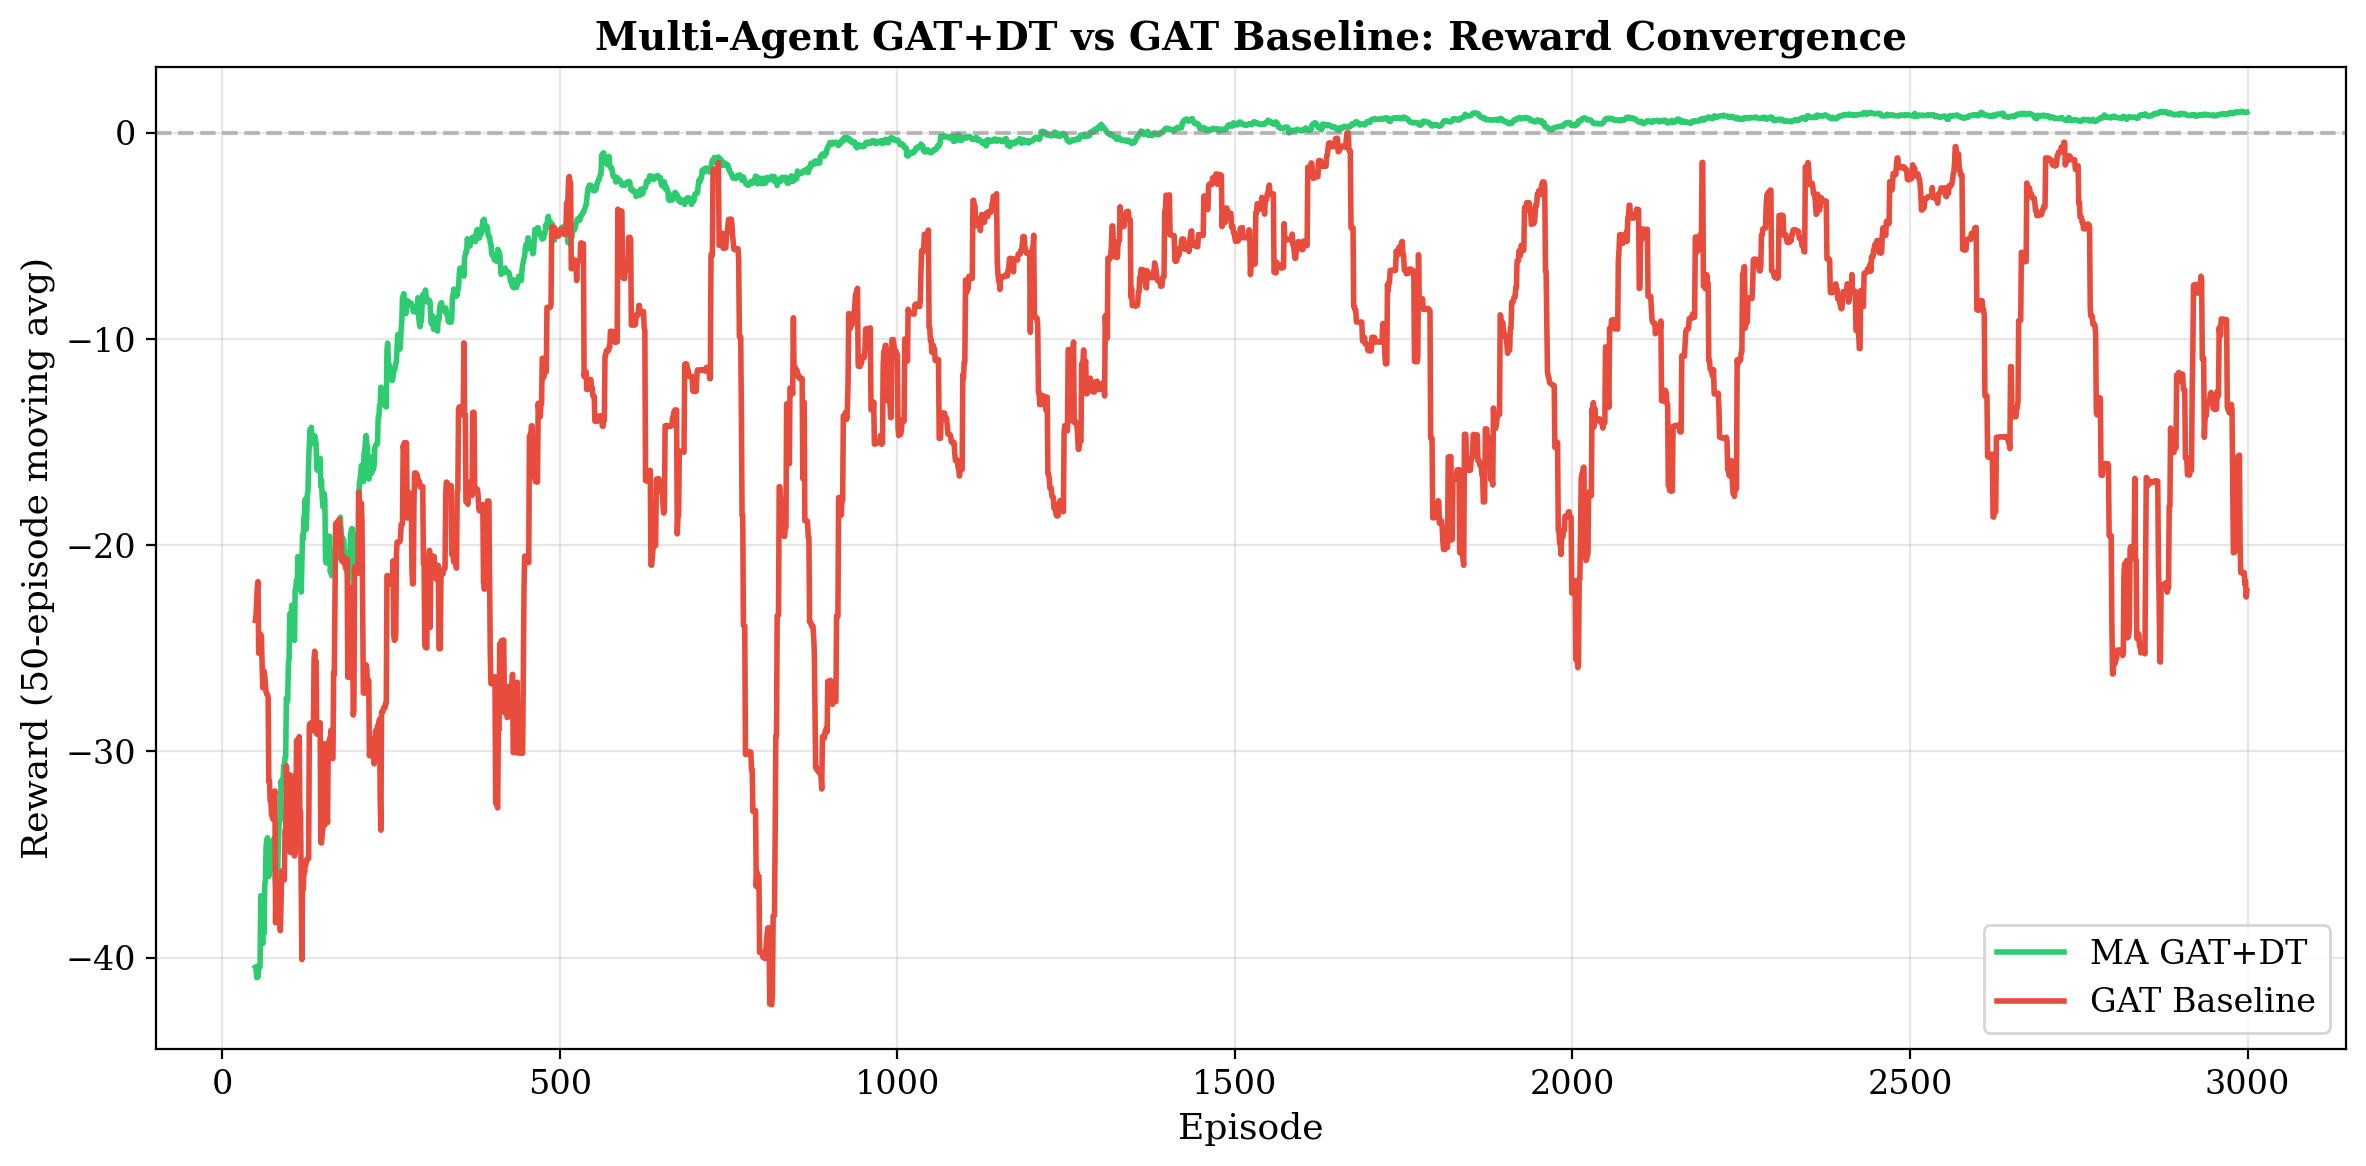
\includegraphics[width=\linewidth]{comparison_reward_graph.png}
  \caption{Reward convergence over 3,000 episodes: MA GAT+DT (green) vs.\ GAT Baseline (red), 50-episode moving average.}
  \label{fig:reward}
\end{figure}

\subsection{Path Efficiency and End-to-End Latency}

The MA GAT+DT was able to achieve an average path length of $3.67$ hops, compared to $50.85$ hops obtained by the GAT Baseline. This indicates a saving of $47.18$ hops on average for each episode. This shows that the cooperative agents, who use the features provided by the Digital Twin such as jamming probability and node load, are able to detect the shortest paths. This is because the number of relay nodes is reduced, thereby reducing the overall latency. This is because the queuing time and the overall probability of loss are reduced.
However, the GAT Baseline, not having the knowledge of the nodes, sends the traffic through the longer paths, thereby increasing the overall transmission time. By having the knowledge of the paths, the 50 agents that cooperate to send the traffic through the network using the proposed MA GAT+DT are able to send the traffic effectively, thereby avoiding the overloaded nodes.

\subsection{Jamming Avoidance and Network Robustness}

The Average Jammed Steps metric indicates the efficiency of the jamming probability factor in the cooperative routing process. In the model, the MA GAT+DT reduced the average jammed steps from $1.25$ to $0.29$, representing a $76.8\%$ decrease.
This significant reduction demonstrates the model's proactive approach to avoiding interference zones and unreliable nodes through the use of the Digital Twin, thereby ensuring the reliability of the link and the stability of the communication process despite the presence of adversarial conditions. The context of the model's application to 50 agents at the same time, thereby distributing the results across all active routing paths, further validates this achievement.
\begin{figure}[htbp]
  \centering
  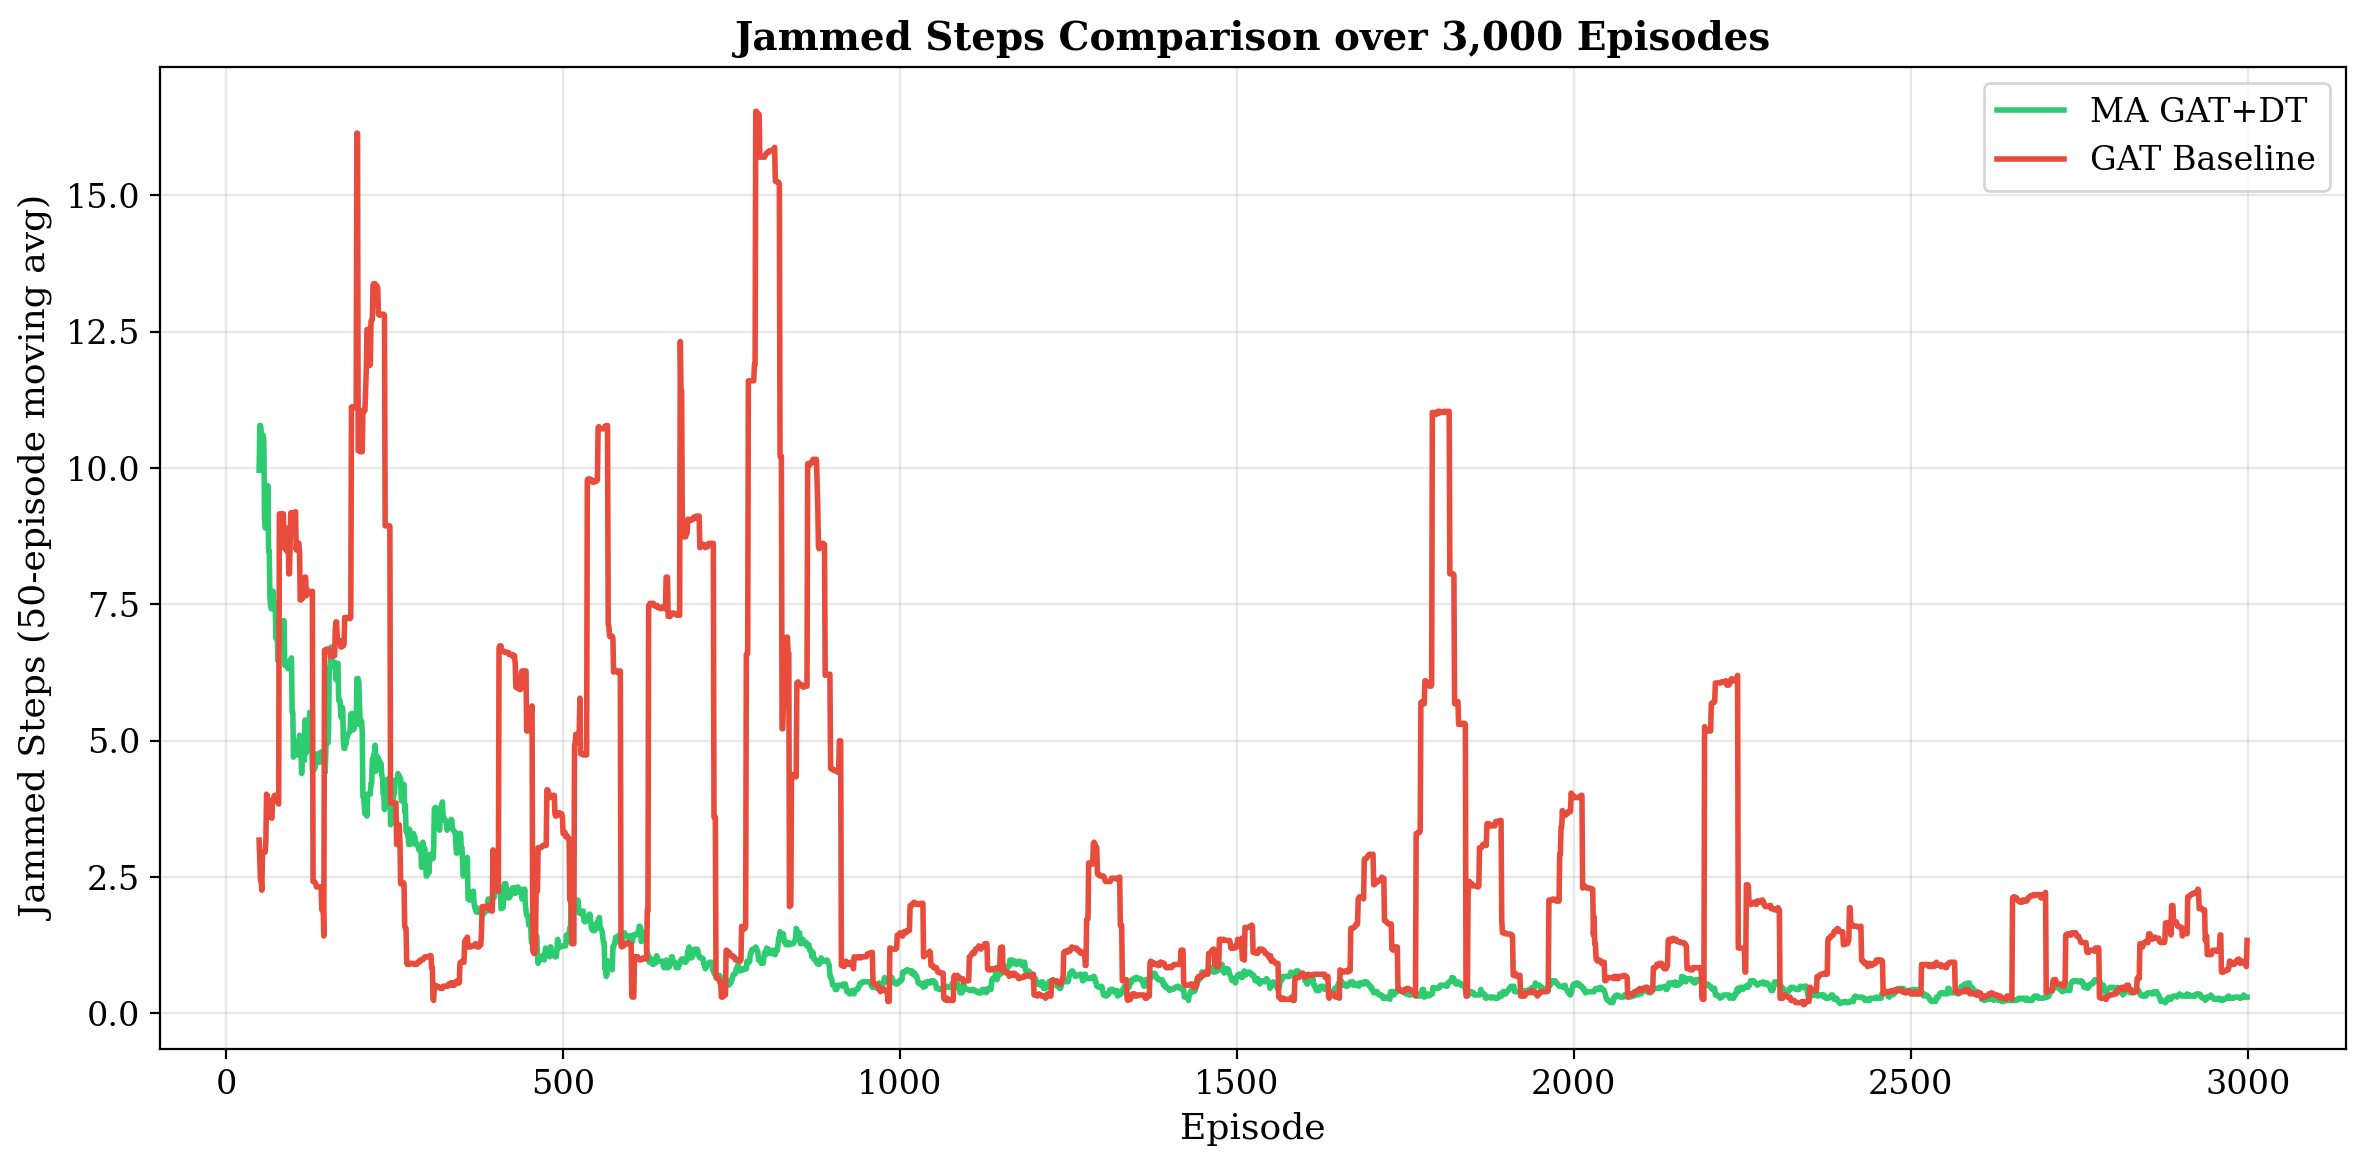
\includegraphics[width=\linewidth]{comparison_jammed_steps_graph.png}
  \caption{Jammed steps comparison over 3,000 episodes: MA GAT+DT maintains near-zero jammed steps while the GAT Baseline shows persistent interference exposure.}
  \label{fig:jammed}
\end{figure}

\subsection{Convergence Behaviour and Training Efficiency}

The MA GAT+DT completed 3,000 training sessions in $35.51$ minutes, whereas the GAT Baseline required $75.21$ minutes. This means that the MA GAT+DT was $52.8\%$ faster, a notable improvement given that it was coordinating 50 agents at the same time, each with their own policy network. Despite this, the MA GAT+DT converged faster than the single-agent baseline, which might be attributable to the cooperative agents' shared experience replay mechanism. This enabled the agents to explore the state space more thoroughly at the same time, resulting in faster policy learning as compared to the baseline model.

The MA GAT+DT model achieved a success rate of $100\%$, compared to the baseline model's $93\%$, demonstrating a clear advantage in reliable packet delivery. Furthermore, in all episodes where the MA GAT+DT model succeeds, the outcome is significantly better, with a higher average reward of $+0.93$ compared to the baseline model's average reward of $-17.78$, as well as a shorter average path length of $3.67$ hops compared to the baseline model's average path length of $50.85$. This demonstrates that the MA GAT+DT model makes significantly better routing decisions than the baseline model across all measured performance indicators.
\begin{figure}[htbp]
  \centering
  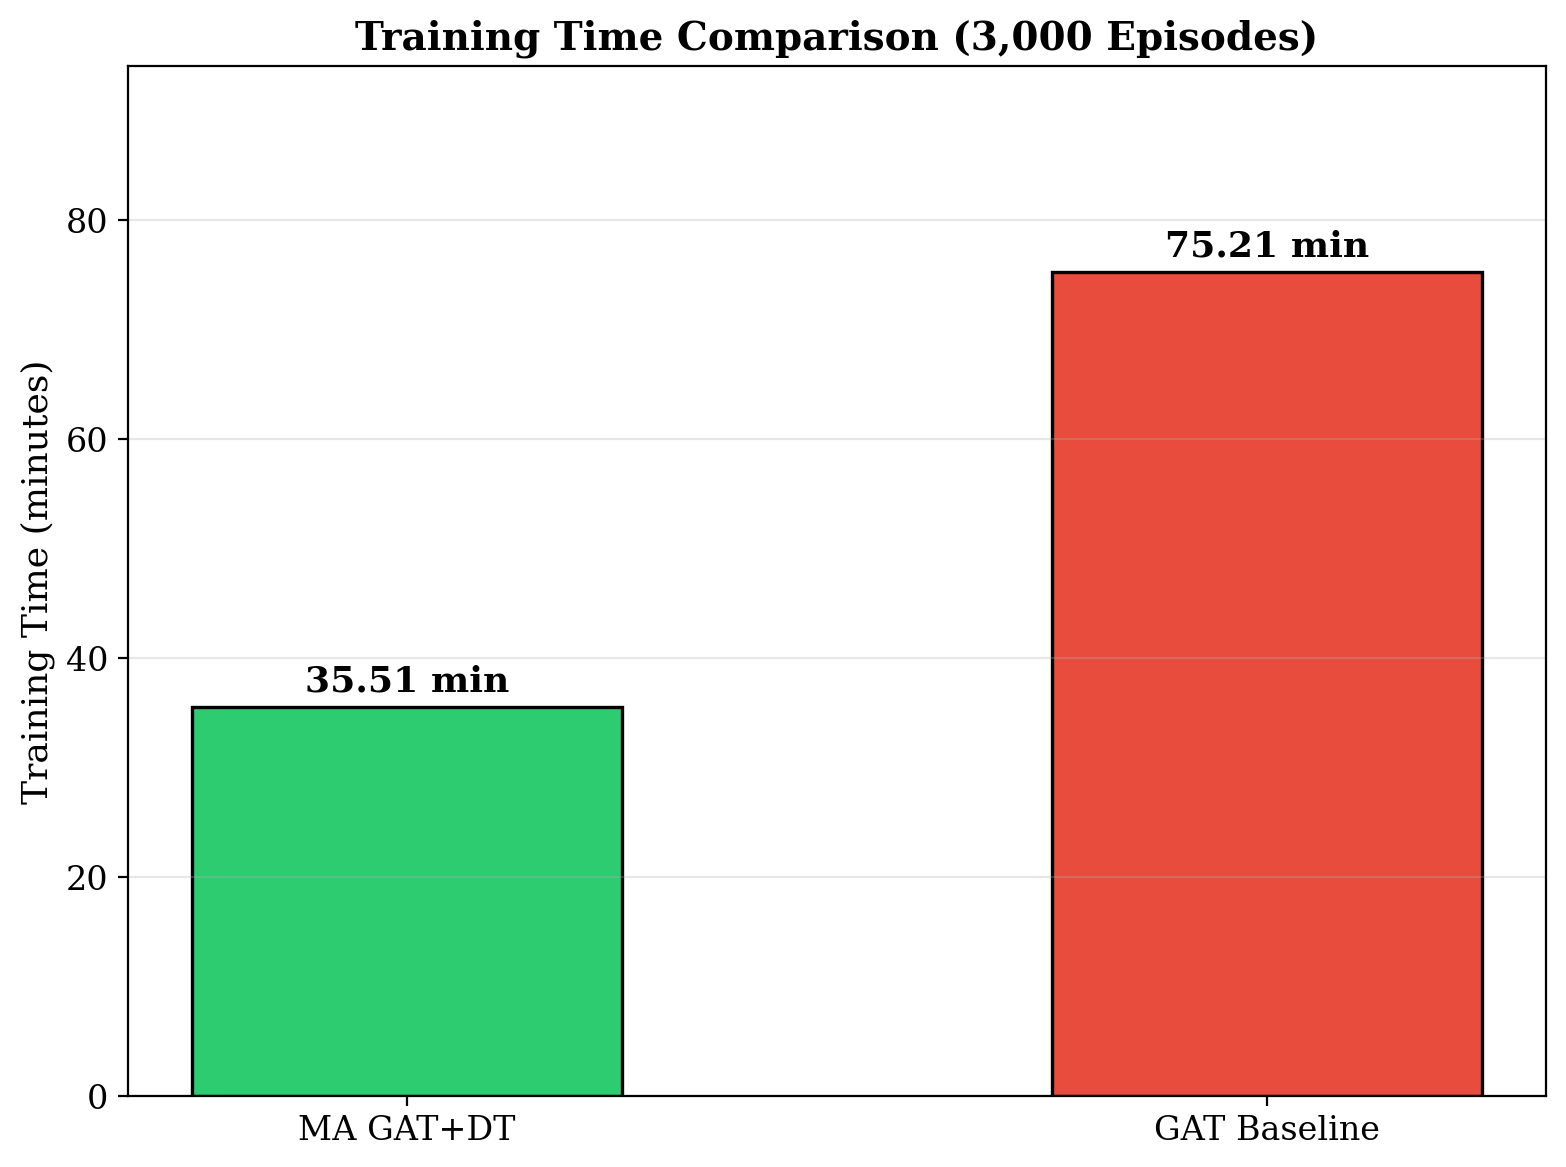
\includegraphics[width=0.85\linewidth]{comparison_time_graph.png}
  \caption{Training time comparison for 3,000 episodes: MA GAT+DT (35.51 min) vs.\ GAT Baseline (75.21 min).}
  \label{fig:training_time}
\end{figure}

\subsection{Success Rate and Reliability}

The MA GAT+DT achieves a success rate of $100\%$, compared to $93\%$ for the GAT Baseline, demonstrating a clear lead in reliable packet delivery. More important is the quality of the route when the model succeeds, and here, the MA GAT+DT far outperforms the GAT Baseline. It achieves a far greater average reward of $+0.93$ compared to the baseline's $-17.78$, achieves routes that are nearly 14 times shorter, and has significantly less interference on the route. The baseline's longer routes are less efficient and more interference prone, resulting in both a lower success rate and poorer route quality. The MA GAT+DT, with its cooperative multi-agent architecture and Digital Twin awareness, has already learned high-quality routing policies that outperform the baseline across every measured metric. These strong routing advantages are expected to be maintained and further reinforced with additional training.
%------------------------------------------------------------------
\section{Conclusion}

This paper proposes an integrated resilience architecture that leverages Digital Twin modelling, Graph Attention Networks, and Multi-Agent Deep Q-Networks for adaptive, jamming-aware routing in Wireless Mesh Networks. The proposed MA GAT+DT model significantly outperformed the GAT Baseline across 3,000 training episodes while converging 52.8\% faster.
Future work may explore integrating transfer learning to enable the trained MA GAT+DT model to generalize across multiple wireless mesh topologies without retraining from scratch. Furthermore, deploying this framework on real hardware testbeds with live radio interference would validate the Digital Twin's accuracy and practical usefulness beyond simulation.


%------------------------------------------------------------------
\begin{thebibliography}{00}

\bibitem{pappone2023}
A.~Pappone \textit{et al.}, ``Graph Neural Network and Multi-Agent Deep Reinforcement Learning for Adaptive Routing in Wireless Mesh Networks,'' 2023.

\bibitem{jin2025}
Z.~Jin, H.~Xu, Z.~Kong, and C.~Pan, ``A Resilient Routing Strategy Based on Deep Reinforcement Learning for Urban Emergency Communication Networks,'' \textit{IEEE Trans. Veh. Technol.}, 2024/2025 (pre-print).

\bibitem{kipf2017}
T.~N.~Kipf and M.~Welling, ``Semi-Supervised Classification with Graph Convolutional Networks,'' in \textit{Proc. ICLR}, 2017.

\bibitem{velickovic2018}
P.~Veli\v{c}kovi\'{c} \textit{et al.}, ``Graph Attention Networks,'' in \textit{Proc. ICLR}, 2018.

\bibitem{krause2023}
A.~Krause, M.~D.~Khursheed, P.~Schulz, F.~Burmeister, and G.~Fettweis, ``The Digital Twin of the Radio Environment: A Novel Approach for Anomaly Detection,'' \textit{IEEE Commun. Mag.}, 2023.

\bibitem{meenakshi2023}
S.~Meenakshi and R.~Shriram, ``Enhancing Fault Tolerance in WMNs Through Adaptive and Resilient Routing Protocols,'' in \textit{Proc. 2023 Int. Conf. Data Sci., Agents \& Artif. Intell. (ICDSAAI)}, IEEE, 2023.

\bibitem{koutsonikolas2024}
D.~Koutsonikolas \textit{et al.}, ``Asynchronous and Distributed Self-Healing for Mesh Networks,'' \textit{IEEE/ACM Trans. Netw.}, 2024 (pre-print).

\bibitem{rajesh2020}
M.~Rajesh and G.~A.~S.~Kumar, ``A Robust Design of Fault Nodes Identification and Recovery Model over Wireless Sensor Network,'' \textit{Wireless Pers. Commun.}, Springer, 2020.

\bibitem{zhang2023}
Y.~Zhang \textit{et al.}, ``Few-Shot Transfer Learning-Based Fault Classification in Wireless Sensor Networks,'' \textit{IEEE Trans. Instrum. Meas.}, IEEE, 2023.

\bibitem{sun2022}
Y.~Sun, M.~Bennis \textit{et al.}, ``Multi-Agent Reinforcement Learning for Dynamic Topology Optimization of Mesh Wireless Networks,'' \textit{IEEE Trans. Commun.}, IEEE, 2022.

\bibitem{menaria2022}
V.~K.~Menaria, S.~C.~Jain, N.~Raju, R.~Kumari, A.~Nayyar, and E.~Hosain, ``NLFFT: A Novel Fault Tolerance Model Using Artificial Intelligence to Improve Performance in Wireless Sensor Networks,'' \textit{IEEE Access}, vol.~8, 2022.

\bibitem{prasad2023}
R.~Prasad and R.~K.~Baghel, ``A Distributed Self-Detection Based Fault Diagnosis for Wireless Sensor Networks,'' \textit{Ad Hoc Netw.}, vol.~149, Elsevier, 2023.

\bibitem{liu2022}
Q.~Liu, L.~Cheng, A.~L.~Jia, and C.~Liu, ``Deep Reinforcement Learning for Intelligent Flow Control in Wireless Mesh Networks,'' in \textit{Proc. IEEE Int. Conf. Commun. (ICC)}, IEEE, 2022.

\bibitem{chen2024}
Y.~Chen, X.~Xu, J.~Li, and H.~Wu, ``Adaptive Fault-Tolerant Routing Using Federated Reinforcement Learning in Wireless Mesh Networks,'' \textit{IEEE Internet Things J.}, vol.~11, no.~4, pp.~5123--5137, Apr. 2024.

\bibitem{lanka2023}
V.~Lanka, ``Multi-Agent Reinforcement Learning (MARL),'' \textit{Medium}, 2023. [Online]. Available: \url{https://vinaylanka.medium.com/multi-agent-reinforcement-learning-marl-1d55dfff6439}

\end{thebibliography}

\end{document}
